\chapterimage{chapter_head_1.png}

\chapter{Theorembeweiser}
\section{Einleitung}
Der Eine kennt sie überhaupt nicht, der Andere womöglich noch aus der Schule, aber wirklich
jeder Student mit Mathematikkursen kennt sie - die Beweise.
In der Mathematik werden seit jeher Theorien aufgestellt, bewiesen und mitunter auch wiederlegt.
Man kann das Beweisen dieser als eine Art Kunstform ansehen.
So gibt es häufig nicht nur den einen Weg zum Ziel, sondern oftmals auch schnellere, schönere und/oder einfachere.
Allen gemein ist allerdings, dass Außenstehende damit kaum etwas anfangen können. Nichts desto trotz resultieren die Bemühungen der Mathematiker nicht zuletzt in einen sichtbaren Nutzen.
Als ein Beispiel sei hierbei das vier Farben Problem genannt. Kurz und knapp geht es um die Frage: \enquote{Ist es möglich eine Landkarte mit lediglich vier verschiedenen Farben so einzufärben, so das am Ende alle benachbarten Länder verschiedenfarbig sind?}
Die Frage entstand bereits im 19. Jahrhundert, als das Drucken von zusätzlichen Farben noch mit erhöhtem Aufwand einher ging. 1852 formulierte Francis Guthrie erstmals dazu einen Satz als Vermutung. Dieser erlangte schnell Popularität und es folgten eine Reihe von Beweisen, welche dann früher oder später wiederlegt wurden. Erstmals bewiesen wurde er 1976 von Appel und Haken, welche zu jener Zeit frisch entwickelte Methoden zum computergestützten Beweisen von Theoremen anwendeten. Dazu wurde das Problem zunächst auf die Ebene der Graphentheorie getragen und anschließend mit einer Mischung aus klassischen und computerbasierten Beweisen zu einem positiven Ergebnis gebracht. Das allgemeine Problem wurde dabei auf 1936 Fälle (später 1478) reduziert, welche der Computer dann einzeln durchprüfen konnte. Es gibt vor allem zwei Hauptkritikpunkte an Appel und Hakens Beweis:
\begin{enumerate}
\item Es wurde ein Computer benutzt, sodass nicht alles verifiziert werden kann.
\item  Gerade der Teil, der per Hand geprüft werden müsste, ist so kompliziert und
mühsam, dass ihn, soweit bekannt, niemand unabhängig geprüft hat.
\end{enumerate}
Man wird schnell bemerken, dass dies ein durchaus stark diskutiertes Thema ist. So argumentieren Kritiker, dass Beweise stets von Menschenhand nachprüfbar und nachvollziehbar sein sollten oder zweifeln gar die Korrektheit der maschinellen Beweise an. Nun, in der Tat verstecken sich häufig Fehler in Computerprogrammen, sodass die verwendeten Algorithmen mitunter inkonsistent arbeiten. 1996 bewiesen N. Robertson, D. P. Sanders, P. Seymour und R. Thomas den Vier-Farben-Satz mit der gleichen Beweisidee, reduzierten allerdings die Anzahl der Problemfälle auf 633. Mittlerweile gibt es noch weitere unabhängige Beweise dazu. Man kann zwar nicht ausschließen, dass der Mensch oder die Maschine in einem geführten Beweis Fehler gemacht haben, aber je häufiger ein Theorem unabhängig bewiesen wird, desto
unwahrscheinlicher wird es, dass all diese Beweise fehlerhaft sind. Anhand der folgenden Tabelle von Thomas C. Hales[] sieht man, dass es seit längerem Bestrebungen gibt, mathematische Aussagen mit dem Computer zu beweisen.

\begin{table}
\begin{tabular}{ccccc}
\toprule
Jahr & Theorem & Beweissystem & Formaler Beweis & Klassischer Beweis \\ \midrule
1986 & First Incompleteness & Boyer-Moore & Shankar & Gödel \\
1990 & Quadratic Reciprocity & Boyer-Moore & Russinoff & Eisenstein \\
1996 & Fundamental - of Calculus & HOL Light & Harrison & Henstock \\
2000 & Fundamental - of Algebra & Mizar & Milewski & Brynski \\
2000 & Fundamental - of Algebra & Coq & Geuvers et al. & Kneser \\
2004 & Four-Color & Coq & Gonthier & Robertson et al. \\
2004 & Prime Number & Isabelle & Avigad et al. & Selberg-Erdös \\
2005 & Jordan Curve & HOL Light & Hales & Thomassen \\
2005 & Brouwer Fixed Point & HOL Light & Harrison & Kuhn \\
2006 & Flyspeck I & Isabelle & Bauer-Nipkow & Hales \\
2007 & Cauchy Residue & HOL Light & Harrison & classical \\
2008 & Prime Number & HOL Light & Harrison & analytic proof \\
\bottomrule
\end{tabular}
\end{table}

Darüber hinaus haben sich über die Jahre hinweg verschiedene Systeme und auch verschiedene Anforderungen an diese entwickelt.
Im folgenden möchte ich erklären was Theorembeweiser (kurz TB) sind, wie diese arbeiten und wofür wir sie brauchen.
Dazu werden der formale Beweis, Erfüllbarkeitsprobleme (kurz SAT, engl. für \enquote{satisfiability}), interaktive TB und automatisierte TB vorgestellt und zum Schluss gibt es einen Ausblick auf die Anwendungen und zukünftige Bestrebungen.

\section{Der formale Beweis}
Klassische Beweise sind in der Regel so gehalten, dass Mathematiker diese gut
verstehen bzw. nachvollziehen können. Hinter Bezeichnungen und Abkürzungen
verstecken sich dabei häufig sehr spezielle mathematische Ausdrücke in Form von
Eigenschaften und Formeln, welche der Laie ohne Frage als Fremdsprache
identifizieren kann. Darüber hinaus führen Mathematiker Beweise häufig
schemenhaft oder auch anhand von Beispielen, die dann verallgemeinert werden
können. So kommt es nicht selten vor, dass für eine Aussage mehrere Fälle gezeigt
werden müssen, aber nur einer mit dem Zusatz vorgerechnet wird, dass die anderen
Fälle analog behandelt werden. Ebenfalls gern verwendet werden Formulierungen wie
\enquote{Ohne Beschränkung der Allgemeinheit} (kurz OBdA) oder \enquote{Trivial}, deren
Bedeutung dem Mathematiker klar ist. Der klassische Beweis erfordert auch häufig
kreative Wege und Beweisideen, die mitunter erst nach einigem Probieren, etwa
umformen und umbenennen, ersichtlich werden. Ein formaler Beweis hingegen
umfasst alles. Jede Implikation muss auf ihre Gültigkeit geprüft und jeder logische
Schritt, bis zurück zu den fundamentalen Axiomen der Mathematik, muss vorhanden
sein. Um zum Beispiel zu zeigen, dass ein Graph planar ist, reicht es dem
Mathematiker, wenn der Graph entsprechend gezeichnet werden kann. Im formalen
Beweis würde eine zusammenhängende Argumentationskette entstehen, die den
theoretischen Kontext vollkommen abdeckt. Wie man sich leicht überlegt wird so
etwas leicht unüberschaubar und umfangreich. Um dies ein wenig zu verdeutlichen
möchte ich einen computergefertigten formalen Beweis vorstellen ohne dabei auf den
mathematischen Hintergrund einzugehen.
Als Beispiel sei die Robbins Algebra gewählt. Der Computer hat damals fast 8 Tage gebraucht um diese Lösung zu ermitteln. Brandon Fitelson benutz in seiner Arbeit \enquote{Using Mathematica to Understand the Computer Proof of the Robbins Conjecture}~\cite{robinsconjecture} eine andere Darstellungsform um den Beweis übersichtlicher und nachvollziehbarer zu gestalten.
Er bemerkt, dass es trotzdem an einigen Stellen äusserst schwierig ist, zu verstehen, wie tatsächlich vorgegangen wird.
Interessierten an den mathemathischen Aspekten empfehle ich daher seine Aufarbeitung.
Er nutzt die klassische Notation, in der die Negation in der typischen Boolschen schreibweise dargestellt wird, wodurch dem Betrachter einige Erleichterung beim lesen verschafft wird.
Ich zeige an dieser Stelle den eigentlichen Beweis von W. McCun, welcher mit dem Equational Theorem Prover (kurz EQP, ein automatisierter Theorembeweiser) angefertigt wurde und im Anschluss folgt eine aufgearbeitete Fassung von Thomas C. Hales~\cite{hales_formalproof}, in der übersichtlich zwischen Umformungen, Substitutionen und Anwendungen der Robbins Identität unterschieden wird.

Um beide Notationen in Einklang zu bringen sei gesagt, dass   $n(\ldots)$, $[\dots]$ und $\bar(x)$ die Negation darstellen und die Verknüpfung $(x,y) \rightarrow x + y$ aus dem 1. Teil durch $(x,y) \rightarrow xy$ in Hales Aufarbeitung ersetzt wurde.
Der direkte Vergleich dieser beiden Beweise zeigt eindeutig, dass der
Computerbeweis mitunter sehr schwer zu lesen ist und durchaus unhandlich sein
kann. Heutzutage wird daher immer häufiger auf interaktive Beweise und vor allem
auch eigene Ausgabestrukturen gesetzt, wie z.B. Isar (der Beweissprache von
Isabelle). Nach Möglichkeit sollen diese sowohl der Maschine als auch dem Menschen
ermöglichen, die Sprache gut zu lesen und zu verstehen.
Wir können diesen formalen Beweis nun als das Endergebnis verstehen, welches wir hier sehen, eine Kette von logischen Inferenzschritten.

\section{SAT / SMT}
Hinter einem Erfüllbarkeitsproblem versteckt sich die Frage, ob es für eine aussagenlogische Formel eine Lösung gibt. Man stelle sich jetzt eine einfache
mathematische Ungleichung vor, wie zum Beispiel $3+7<2*x$. Auf die Frage ob eine natürliche Zahl x existiert, welche diese Formel erfüllt, werden die meisten im Schlaf
eine Antwort geben können. Solche Formeln müssen natürlich nicht auf die natürlichen Zahlen, ja geschweige denn auf die Mathematik beschränkt sein.
Um eine Maschine anleiten zu können Theorien, bzw. Aussagen auf ihre Gültigkeit hin zu überprüfen oder gar diese zu beweisen, muss zunächst eine Struktur
gefunden werden, auf deren Grundlage der Computer entscheiden kann, wann eine Aussage wahr oder falsch wird, eine Sprache. Ohne zu sehr ins Detail gehen zu
wollen, sei an dieser Stelle gesagt, wir benötigen eine Prädikatenlogik. SAT formalisiert dieses Thema und führt Theorien ein, mithilfe derer wir die Aussagen
logischer Konstruktionen, umformen bzw. Belegungen finden können, um diese zu lösen.
Die \enquote{Satisfiability Modulo Theories}, kurz SMT, erweitert dieses System um die Möglichkeit Formeln und Terme um spezielle theoretische Aussagen zu erweitern.
Dies sind in der Regel Terme, welche dann von dem SMT-Löser selbst gar nicht verarbeitet werden können und dessen Wahrheitsgehalt von einem sogenannten
Theorie-Löser ermittelt werden muss. Bei den automatischen Theorembeweisern werde ich noch einmal darauf zurück kommen.
Zusammenfassend ist SAT also die Theorie von der Lösbarkeit prädikatenlogischer Formel und Terme und SMT eine Erweiterung dieser, durch theoretischen Kontext zunächst ungebundener Natur. Im TB stellt dieses Thema die Schnittstelle zwischen der Formulierung des Problems und deren Lösung dar.

\section{Theorembeweiser}
Wir unterscheiden vor allem zwei Sorten von Löser, die interaktiven und die automatisierten, wobei die Interaktiven heutzutage ebenfalls Methoden mitbringen, welche selbstständig nach dem nächsten Umformungsschritt suchen können. Der offensichtlichste Unterschied ist, dass die Automatisierten, wie der Name schon sagt, automatisch nach einer Lösung suchen. Das Programm wird mit allen nötigen Informationen gefüttert und den Rest übernimmt die Maschine.

\subsection{Interaktive Theorembeweiser}
Sie werden auch gerne Beweisassistenten genannt, da sie den Rahmen stellen um geordnet Beweise anzufertigen. Auf der einen Seite prüfen sie alle Inferenzschritte, können aber auf der anderen Seite auch eigenständige Lösungen mit einbringen. Ebenfalls hilfreich ist, dass sie dem Anwender aufzeigen an welchen Stellen noch Unklarheiten bestehen und welche Aussagen noch gezeigt werden müssen. Ein Nachteil ist, dass solche Beweiser zumeist ein hohes Maß an Verständnis für das Programm und seine Sprache vorraussetzen. In der Regel nutzen sie Logiken höherer Ordnung (kurz HOL, engl. \enquote{higher order logic}). Als Beispiele für diese Art der Beweiser möchte ich HOL Light, PVS, Coq, Mizar und Isabelle nennen.
Im folgenden sehen wir 2 exemplarische Beweise mit Isabelle. Der Erste wird veranschaulicht, wie mit sogenannten \enquote{apply}-Scripts gearbeitet wird, das Zweite, wie mit Isar eine lesbare Form erreicht wird.
Ursprünglich sollte hier ein eigenes kleines Beispiel in der zweiten Variante ausformuliert und mit allerhand Erklärungen ausgeschmückt werden, allerdings sprengt dies den Rahmen, sodass hier lediglich die Kenntnis von den beiden Varianten ausreichen soll.

\subsubsection*{Variante 1}
Gegeben ist eine Listenstruktur mit zwei Funktionen, app und rev. Die Erste soll zwei Listen miteinander verknüpfen, die Zweite die
Reihenfolge umkehren.
Gezeigt werden soll, dass das doppelte Umkehren (der Reihenfolge der Elemente) einer Liste, die ursprüngliche Liste ergibt.
In \cref{fig:isabelle1} sieht man den Kopf des Beweises, mit den Definitionen des Datentyps dieser Listen und der beiden Funktionen app und rev.

Zunächst beginnen wir mit dem Theorem und arbeiten uns dann mit den Lemmas von unten nach oben, immer dann, wenn zusätzliche Aussagen gezeigt werden müssen.
In |1 in \cref{fig:isabelle2} haben wir Isabelle gesagt, dass eine Induktion über die Liste xs durchgeführt werden soll. In \cref{fig:isabelle3} sieht man die Antwort darauf, die zu erfüllenden zwei Ziele:
\begin{itemize}
\item Induktionsanfang und
\item Induktionsschritt.
\end{itemize}
ähnlich sieht es bei den Lemmas aus.
In \cref{fig:isabelle4} sieht man, wie Isabelle den Beweis akzeptiert und eine Regel mit Platzhaltern zur Verfügung stellt, welche nun zur
Vereinfachung genutzt werden kann.
Lemma rev\_app wird für beide Goals vom Theorem rev\_rev gebraucht und die anderen beiden Lemmas für die beiden Goals von rev\_app. \enquote{[sim]} steht hier für eine Vereinfachung, d.h. Isabelle darf die Regeln anwenden um Termumformungen durchzuführen, z.B. durch \enquote{apply(simp)}.

\begin{figure}
\centering
\caption{Isabelle Proof 1}
\label{fig:isabelle1}
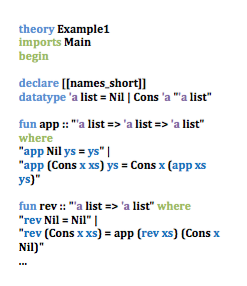
\includegraphics[width=.3\textwidth]{chapters/theoremprovers/isabelle1.png}
\end{figure}

\begin{figure}
\centering
\caption{Isabelle Proof 2}
\label{fig:isabelle2}
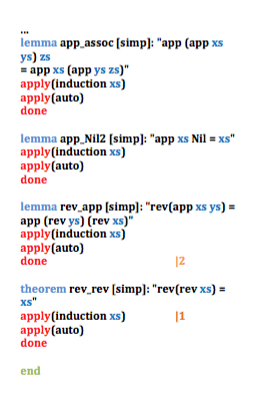
\includegraphics[width=.3\textwidth]{chapters/theoremprovers/isabelle2.png}
\end{figure}

\begin{figure}
\centering
\caption{Isabelle Antworten}
\label{fig:isabelle3}
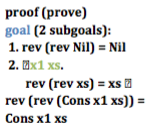
\includegraphics[width=.15\textwidth]{chapters/theoremprovers/isabelle3.png}
\end{figure}

\begin{figure}
\centering
\caption{Isabelle akzeptierter Beweis}
\label{fig:isabelle4}
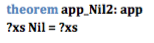
\includegraphics[width=.2\textwidth]{chapters/theoremprovers/isabelle4.png}
\end{figure}

\subsubsection*{Variante 2}
In \cref{fig:isabelle5} sieht man ein Beispiel, in dem der Beweis eigenhändig durchgeführt wird. Gezeigt werden soll, das Abbildungen von einer Menge in ihre Potenzmenge niemals surjektiv sein können. Ohne genau zu wissen wie die neuen Begriffe, wie assume, from, have und show anzuwenden sind, kann man den Beweis doch bereits recht leicht lesen.
In \cref{fig:isabelle6} sieht man, wie sich der Beweisstatus in |3 verändert hat, nach der Annahme, dass f surjektiv sei. Es wird ein f festgehalten, das Goal hat sich nicht verändert.
In \cref{fig:isabelle7} sieht man die Ausgabe von Isabelle, bevor das Lemma akzeptiert wird (|4).

\begin{figure}
\centering
\caption{Isabelle Beweis}
\label{fig:isabelle5}
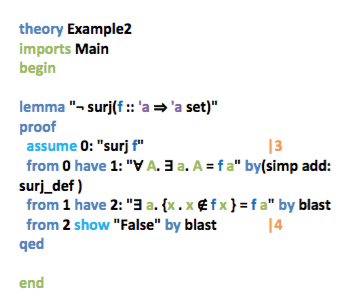
\includegraphics[width=.3\textwidth]{chapters/theoremprovers/isabelle5.png}
\end{figure}

\begin{figure}
\centering
\caption{Isabelle Beweisstatus}
\label{fig:isabelle6}
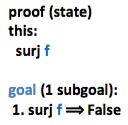
\includegraphics[width=.15\textwidth]{chapters/theoremprovers/isabelle6.png}
\end{figure}

\begin{figure}
\centering
\caption{Isabelle Status vor Lemma}
\label{fig:isabelle7}
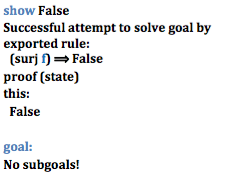
\includegraphics[width=.3\textwidth]{chapters/theoremprovers/isabelle7.png}
\end{figure}

\subsection{Automatisierte Theorembeweiser und DPLL(T)}
Nachdem wir nun die interaktiven Theorembeweiser kennen gelernt haben, schauen
wir uns die automatisierten etwas genauer an.
Wir unterscheiden unter anderem
zwei Methoden bei der automatisierten Beweissuche, den Davis-Putnam-Logeman-Loveland Algorithmus (kurz DPLL, auch DPLL(T) wobei T für Theorie steht) und das
Tableaukalkül (auch Baumkalkül, bzw. engl. Method of analytic tableaux).
Beide Herangehensweisen arbeiten auf einer Prädikatenlogik, allerdings sei das Baumkalkül
nur als weiterer Vertreter mit aufgeführt.
Grundlegend wird bei diesem versucht die
 Gegenaussage zu widerlegen.


\section{Schlusswort}
Nachdem wir nun einen Einblick in der Welt der TB erhalten haben und in Grundzügen wissen was TB sind und wie sie arbeiten sollen folgend einige Anwendungen vorgestellt werden.
Da Computerprogramme in verschiedenen Sprachen geschrieben werden, welche ein Vokabular, eine Grammatik und eine Syntax haben, können diese genauso für den theoretischen Inhalt her halten, wie mathematische Probleme.
Ein Beispiel dafür ist der Beweis des Vier-Farben-Satzes von Neil Robertson, Daniel P. Sanders, Paul Seymour und Robin Thomas, welcher genau genommen zwei Beweise beinhaltet.
Der erste zeigt, das der benutzte Algorithmus richtig arbeitet, also verifiziert die Korrektheit und der zweite, dass das Theorem gilt.
In der Wirtschaft setzt man Theorembeweiser vor allem für die Verifikation von integrierten Schaltkreisen und Prozessoren ein, z.B. um kritische Operationen zu prüfen.
Allerdings finden sie auch in Fachübergreifenden Gebieten ihren Nutzen. Insgesamt scheinen sie bei der Programmverifikation einer zunehmenden Beliebtheit zu unterliegen.
Der seL4 Mikrokernel, welcher in unzähligen Mobilgeräten vorkommt, wurde zum Beispiel mithilfe von Isabelle geprüft und seine Korrektheit nachgewiesen.
In der Mathematik sind sie noch sehr umstritten und auch wenn die vorhandenen Beweiser mächtige Werkzeuge sind, so können sie ihren menschlichen Kollegen heute noch nicht das Wasser reichen.
Eine naheliegende Anwendung diesbezüglich wäre nämlich das Erschaffen von neuen Theoremen und dabei bringen sie höchstens Triviale Aussagen zustande.
Mit \enquote{Automated Theorem Discovery}~\cite{Gao2014} richtet man den Blick auf das Schaffen von neuem Wissen, was allerdings noch in den Kinderschuhen steckt.
Das sogenannte \enquote{Theory-Exploration} hingegen versucht Möglichkeiten zu verwirklichen, um dem Anwender von interaktiven TB, im Falle des Feststeckens, mit Lemmas und Ideen weiter zu helfen.
Man bedenke, heutige TB zeigen nur, was noch nicht bewiesen ist und nicht, wie man solches zeigen kann.
Als Fazit kann man sagen, dass mit dieser Arbeit die Themengebiete gerade einmal angekratzt werden konnte, denn es gibt noch mehr als genug Ungesagtes zu den Theorembeweisern.
Mir persönlich hat die Arbeit von Thomas C. Hales über den Formalen Beweis sehr gut gefallen, da sie zeitgleich einen guten überblick verschafft.
Ich hatte darüber hinaus ein großes Interesse daran Isabelle einmal kennenzulernen und einen interaktiven TB selbst auszuprobieren.
Auch wenn die Zeit nicht gereicht hat um elegante Beweise zu führen, so konnte man doch zumindest einen Eindruck gewinnen.
Der Internetauftritt von Isabelle~\cite{isabellewebpage} bietet diesbezüglich gut verständliche Tutorials an, die für Interessierte in jedem Fall empfehlenswert sind.
